\documentclass[11pt]{extarticle}
\usepackage{manualdoprofessor}
\usepackage{fichatecnica}
\usepackage{lipsum,media9,graficos}
\usepackage[justification=raggedright]{caption}
\usepackage[one]{bncc}
\usepackage[ubu]{../edlab}

\begin{document}


\newcommand{\AutorLivro}{Charles Darwin}
\newcommand{\TituloLivro}{A origem das espécies}
\newcommand{\Tema}{História da ciência}
\newcommand{\Genero}{Tratado científico}
\newcommand{\imagemCapa}{./images/PNLD0060-01.png}
\newcommand{\issnppub}{---}
\newcommand{\issnepub}{---}
% \newcommand{\fichacatalografica}{PNLD0060-00.png}
\newcommand{\colaborador}{{Vicente Castro e Bruno Gradella}} 


\title{\TituloLivro}
\author{\AutorLivro}
\def\authornotes{\colaborador}

\date{}
\maketitle



%\baselineskip=1.20\baselineskip\par



\begin{abstract}\addcontentsline{toc}{section}{Carta ao professor} 

Nascido em 1809 em Shrewsbury, Grã Bretanha, Charles Darwin foi um naturalista,
geólogo e biólogo. Em 1831, partiu numa viagem pelas costas da América do Sul,
África e Austrália, com a missão de observar e coletar amostras de seres vivos
desses lugares. Tornou-se um dos cientistas mais importantes do Ocidente pela
sua teoria sobre a evolução dos seres vivos, que defendia que todos os seres
vivos descendem de um ancestral em comum e que os ramos evolutivos são
resultados da seleção natural. Segundo o biólogo, o meio e as condições
selecionam os indivíduos mais adaptados para sobreviverem e procriarem, onde os
seres menos habilitados são eliminados.

Apesar de ser um trabalho científico, \emph{A origem das espécies}, publicado
pela primeira vez em 1859, tem o diferencial de ser uma obra direcionada ao
público leigo.  Por isso, rapidamente o livro tornou-se um sucesso, e, a teoria
da seleção natural nele veiculada, uma controvérsia. Afinal, ele ia contra não
só os clássicos da ciência, mas também as versões da Bíblia sobre o surgimento
e o desenvolvimento da vida na Terra.  Nesta obra, Darwin irá responder
perguntas como ``por que novas espécies aparecem?'', ``por que essas espécies se
modificam no decorrer do tempo?'', que surgiram durante sua viagem no navio da
Coroa Britânica. 

Esta edição traz, além do texto integral, quatro outros textos com os
acréscimos mais importantes das edições posteriores, e as primeiras reações do
mundo científico à obra. 

Esperamos que as indicações propostas aqui neste manual sejam muito úteis no
trabalho em sala de aula!

\end{abstract}


\tableofcontents

\section{Introdução}

Teriam os seres vivos surgido com a complexidade que apresentam hoje, ou teriam
eles se transformado no decorrer do tempo?
Durante milênios, filósofos e naturalistas debateram esse tema.
Esse livro é considerado a base da biologia evolutiva que redefiniu para sempre
a ciência moderna. Publicado em 1859, a obra apresenta a teoria de Darwin com base em dados coletados ao longo de sua jornada na expedição Beagle. 


Desde muito jovem, já demonstrava seu amor pela ciência, dedicando-se às suas
coleções e realizando experimentos com seu irmão, em um laboratório de
química. Aos 16 anos, Darwin iniciou o curso de medicina,  seguindo uma tradição de família, mas acabou abandonando o curso.

Com muito custo, formou-se em teologia, para se tornar um clérigo.  Mas foi uma
viagem de cinco anos que definiu o futuro do jovem.  Em 1831, Darwin embarcou
no Beagle (ver fig.\,\ref{fig:PNLD0060-21}), um navio enviado pela coroa britânica para atualizar os mapas das costas da América do Sul,  África e Austrália.
As pesquisas e estudos feitas pelo naturalista durante a viagem a bordo do
Beagle fundamentaram sua teoria da evolução.


A função do jovem era observar e coletar amostras de seres vivos desses
lugares. A viagem durou 
durou cinco anos, durante a qual Darwin aplicou parte do conhecimento que tinha sobre a criação de animais, observando que, dadas condições ideais, todos os animais em cativeiro
sobrevivem. Ele sabia que um criador de animais pode selecionar indivíduos com as características que mais lhe interessam para se reproduzir.
Foi assim que se criaram as diferentes raças (subespécies) de galinhas, pombos
e porcos. E de o homem é capaz de fazer essa seleção artificial, então a natureza deve fazer a própria seleção natural.

Em resumo, pelo darwinismo, os seres vivos se desenvolvem com base na variação,
adaptação e seleção natural das espécies, em um processo de longo prazo.
Os indivíduos nascem com pequenas diferenças e algumas delas facilitam sua
sobrevivência.

Ao se reproduzirem, esses indivíduos transmitem a característica favorável
a seus descendentes. O meio ambiente não induz a nenhuma variação, apenas funciona como filtro que
seleciona os organismos mais adaptados ou mais aptos a sobreviver.

Um dos mais interessantes conceitos de Darwin é o de deriva genética,  mecanismo pelo qual um acontecimento aleatório altera a frequência de
determinado alelo dentro de uma população.

Ainda que trabalhos posteriores tenham complementado a teoria de Darwin,
a precisão com a qual explica e prevê os rumos da evolução mantém sua obra como
extremamente relevante.
Desenvolvimentos na genética e na biologia molecular levaram a algumas mudanças
no entendimento da teoria evolucionista, porém as ideias de Darwin permanecem
até hoje essenciais no campo da biologia.


O livro representa um grande salto científico, consolidando conhecimentos
passados e contemporâneos acerca da biologia.
Também propôs a explicação das razões da diversidade das espécies, ao
dissertar sobre a seleção natural.

À época da morte de Darwin, sua teoria da evolução já era universalmente
aceita. 
Em homenagem ao conjunto de seu trabalho científico, ele foi enterrado na
abadia de Westminster ao lado de reis, rainhas e outras ilustres figuras da
história britânica. 

Darwin foi ao mesmo tempo geólogo, botânico, zoologista e homem de ciência. 
Sua famosa viagem foi uma preparação fundamental para a sua carreira de
pesquisador e escritor. Na introdução de seu livro, ele assim se refere:  

\begin{quote}
As relações
geológicas que existem entre a fauna extinta da América meridional me
impressionaram profundamente quando da minha viagem a bordo do Beagle, na
condição de naturalista.  Estes fatos parecem lançar alguma luz sobre a origem
das espécies.
\end{quote} 

Darwin reuniu grandes coleções de rochas, plantas
e animais, eres fósseis e vivos que eram enviados à sua pátria. 
Imediatamente após seu regresso à Inglaterra, Darwin iniciou um caderno de
notas sobre a evolução, reunindo dados sobre a variação das espécies,
hoje considerado um esboço de \textit{A origem das espécies}. 

De início, o grande enigma era explicar o aparecimento e o desaparecimento das
espécies. Por que se originavam as espécies? Por que se modificavam com o passar dos tempos? E diferenciavam-se em numerosos tipos e frequentemente desapareciam do mundo por completo?

O gênero textual da obra é o \textit{tratado científico}, uma produção de caráter
técnico, organizada a partir da coleta de dados, de
linguajar específico a determinado campo do conhecimento,  mantendo, contudo,
o caráter público.

Este é um livro base para o entendimento de uma área fundamental da ciência:
a biologia evolutiva. De linguagem acessível, a obra oferece as premissas dos mecanismos de seleção
natural e consequente evolução das espécies.
Além disso, por ser um marco da história da ciência, é uma oportunidade do
leitor vivenciar esse ponto de inflexão no desenvolver científico.

\SideImage{Reprodução do livro de Robert Taylor Pritchett da primeira edição ilustrada de \textit{Murray}, 1890: Beagle no Estreito de Magalhães no Monte Sarmiento no Chile. CC-BY.}{PNLD0060-21}

\Image{Trajeto da viagem da expedição Beagle.}{PNLD0060-20}



\section{Propostas de Atividades I}


\subsection{Pré"-Leitura}

\paragraph{Tema} As origens d'\textit{A origem das espécies}

\paragraph{Conteúdo} Contextualização acerca da vida e do meio social
em que Charles Darwin viveu.

\paragraph{Objetivo} Apresentar aos e às estudantes as condições
que possibilitaram o cientista a desenvolver suas teses, fazendo"-os
refletir sobre as etapas necessárias à construção do trabalho científico
e, consequentemente, desmistificar o senso comum de que se trata de 
um trabalho simples.

\paragraph{Justificativa} Antes de se iniciar a leitura, é conveniente oferecer ao 
aluno um panorama em
relação ao autor da obra, e ao contexto em que ele estava inserido.
Recomenda-se para isso a utilização da metodologia da sala de aula invertida,
no qual os alunos, individualmente, ou em grupos, buscarão informações acerca
de temas que compõem o contexto da obra.

\paragraph{Metodologia}

\begin{enumerate}

	\item
	O professor ou a professora deve separar a turma em cinco grupos. Cada um deve escolher
	um dos itens a seguir para desenvolver uma pesquisa, em fontes abertas e confiáveis.
	São eles: 
	\begin{itemize}
	\item A expansão e a presença do Império Britânico no mundo;
	\item A biografia de Charles Darwin;
	\item A passagem de Charles Darwin pelo Brasil;
	\item Detalhes a respeito das viagens e embarcações utilizadas à época.
\end{itemize}
\BNCC{EM13LP12}
	
	\item
	Num segundo momento, cada grupo deverá fazer uma breve apresentação sobre 
	o item pesquisado, compartilhando os resultados com o restante da turma.
	Estimule questionamentos, como por exemplo: qual é a relação entre
	a expansão do Império Britânico e o desenvolvimento das pesquisas
	que deram no livro de Darwin? 
	\BNCC{EM13LP16}

\end{enumerate}

\paragraph{Tempo estimado} Duas aulas de 50 minutos.


\subsection{Leitura}

\paragraph{Tema} Os nomes das coisas

\paragraph{Conteúdo} Exercício de nomeação científica e poética.

\paragraph{Objetivo} Propor uma reflexão sobre a nomeação no mundo científico
a partir do capítulo 13 da \emph{A origem das espécies} e da interpretação de um poema. 

\paragraph{Justificativa} Todo pensamento científico se vale de um vocabulário muito próprio para
expressar seus objetos de pesquisa e trabalho. Dentro da biologia, não poderia
ser diferente. Nesse campo, é notável o trabalho de Carlos Lineu que, com
a publicação, em 1735, da obra \emph{Systema Naturae}, desenvolveu o sistema de
classificação binomial dos seres, lançando as bases da taxonomia, num formato
até hoje utilizado. O sistema de Lineu era simples, porém muito rico. A ideia
era combinar dois nomes em latim, o primeiro, genérico, escrito com letra
maiúscula, referente ao gênero do indivíduo pertence. O segundo, específico,
escrito com letra minúscula, tangente à espécie. Como exemplo, podemos citar
\emph{Orcinus orca}, orca, \emph{Felis catus}, gato doméstico, \emph{Tibouchina
mutabilis}, manacá-da-serra. Essa iniciativa, teve o intuito de promover uma
maior comunicação entre os cientistas, afinal, nem todos os seres têm o mesmo
nome em todas as culturas do mundo. O mais comum é que cada povo nomeie plantas
e animais de acordo com seu idioma, cultura e cotidiano. Desse modo, como se
pode ver, com esse sistema, é possível classificar todos os seres, agrupando-os
de uma maneira que obedeça a ordem evolutiva, e seja conveniente para o estudo.

O vocabulário é algo muito importante também na poesia. 
Peguemos um pequeno poema do poeta gaúcho Mario Quintana para pensar a respeito disso: 


\textit{Tristeza de escrever}.

\begin{verse}
Cada palavra é uma borboleta morta espetada na página.\\
Por isso a palavra escrita é sempre triste...
\end{verse}


Podemos entender estes versos da seguinte forma: cada vez que o poeta
utiliza uma palavra num poema, ele está delimitando as possibilidades
de sentido. Ou seja, de alguma forma, está pregando a palavra, uma coisa
viva, a uma parede de sentido específica, que é a folha onde o poema é 
escrito. De modo similar, quando um cientista ou um povo dá um nome para todos os 
seres vivos de uma determinada espécie, com a mesma aparência, ele está, conforme
o poeta, pregando uma borboleta morta numa página. 

\paragraph{Metodologia}

\begin{enumerate}

	\item
	Primeiro, é interessante que o professor ou professora faça a leitura do poema
	de Mário Quintana, apresentado na \textbf{Justificativa}, e estimule a discussão
	sobre os nomes que as coisas têm, no sentido de que, se por um lado
	a nomeação possibilita a comunicação e o entendimento entre pessoas
	diferentes, ela limita as possibilidades de significação da coisa que foi nomeada.
	Estimule, na turma, a discussão sobre os prós e os contras de dar nomes
	às coisas.
	\BNCC{EM13LP06}

	\item
	Em seguida, peça aos estudantes que apontem quais as críticas que Darwin faz ao sistema
	de classificação de Lineu no capítulo 13 de \emph{A origem das espécies}.
	Podem realizar uma leitura coletiva do seguinte trecho:

	\begin{quote}
	 Há, por exemplo, uma frase famosa de Lineu, muitas vezes encontrada de forma um tanto enigmática, a qual nos informa que as características não formam um gênero, mas o gênero gera características. Eu acredito que o sistema inclui algo a mais; e que a afinidade dos descendentes -- a única causa conhecida para a semelhança entre os seres orgânicos -- é um vínculo que está escondido por vários graus de modificação, mas que se torna parcialmente revelado a nós por meio das classificações.
	\end{quote}

	\item
	Depois, o professor ou professora deve sugerir a cada aluno que pesquise cinco 
	seres vivos típicos das fauna e flora brasileiras, devendo, em uma folha ou 
	página da web, colar uma foto desse espécime, colocando ao lado informações sobre o 
	mesmo. O nome popular, o nome científico, habitat etc.
	\BNCC{EM13CNT301}

	\item
	Agora, divida os alunos em grupos, e peça para que pesquisem cinco
	seres fantásticos, de histórias em quadrinhos, filmes, mitos, jogos de
	vídeo"-game. Feito isso, cada grupo deve propor nomes para classificá"-los,
	utilizando a metodologia de Lineu.

\end{enumerate}


\subsection{Pós"-Leitura}

\paragraph{Tema} Disseminando o conhecimento

\paragraph{Conteúdo} Preparação de material informativo sobre o conteúdo trabalhado.

\paragraph{Objetivo} Propiciar aos e às estudantes a experiência de articular
uma pesquisa e uma produção audiovisual com fins de divulgação sobre o tema.

\paragraph{Justificativa} Tendo em vista a necessidade de discussões sobre
a disseminação de \textit{fake news} em nossos tempos, uma atividade de pesquisa
e compartilhamento de informações científicas mostra"-se necessária para que,
cada vez mais cedo, estes e estas estudantes entrem em contato com a seriedade
deste grupo de profissionais. 

A atividade científica deve ser levada a sério,
e parte desta abordagem parte de um trato compromissado com o saber científico
por parte daqueles que preparam os resultados de suas pesquisas para
ser compartilhados com o público. Emulando um papel de pesquisadores
e jornalistas ao mesmo tempo, os e as estudantes estarão desenvolvendo
habilidades essenciais para suas formações enquanto cidadãos numa sociedade
democrática. 

\paragraph{Metodologia} 

\begin{enumerate}

	\item
	O professor ou a professora deve pedir que os e as estudantes se organizem em grupos e,
	valendo-se das informações obtidas nas atividades anteriores,
	acrescidas de outras pesquisas, realizem a produção de um material audiovisual,
	podendo este adotar o formato de reportagem, documentário ou \textit{podcast}. Este
	material deve abordar os principais conceitos da Teoria da Evolução, bem como
	outros conhecimentos de biologia e genética, além da própria biografia de
	Darwin, narrando por exemplo:

\begin{itemize} 
	\item O conceito formulado por Darwin; 
	\item A forma como
    o mesmo foi desenvolvido ao longo de sua viagem; 
    \item Abordar pesquisas
    científicas acerca da origem da vida e da evolução das espécies surgidas
    a partir da teoria de Darwin; 
    \item Indicar os motivos pelos quais as
 	descobertas com a genética consolidaram a Teoria da Evolução; 
 	\item Como
	a evolução funciona? Quais são os processos de seleção natural e artificial?
\end{itemize}
\BNCC{EM13LP17}

\end{enumerate}


\section{Propostas de Atividades II}

A obra \emph{A origem das espécies} possibilita trabalhos interdisciplinares
e integradores de diferentes campos do saber e áreas de conhecimento. A seguir,
propomos algumas atividades que podem ser desenvolvidas conjuntamente com
professores de outras áreas. 

\subsection{Pré"-Leitura}

\paragraph{Tema} A ciência da observação

\paragraph{Conteúdo} Apresentação dos métodos primordiais de pesquisa
científica.

\paragraph{Objetivo} Propiciar aos e às estudantes uma atividade de campo
na área das ciências naturais tendo como ponto de partida a observação
e posterior anotação dos dados observados, em forma de escrita, desenho,
fotografia ou vídeo. 

\paragraph{Justificativa} Dentro da história das ciências biológicas, grandes teorias e propostas
científicas surgiram de estudos de campos e pesquisas empíricas de grandes
naturalistas. Nessas empreitas, muitos deles realizavam desenhos para catalogar
animais e plantas desconhecidos, atentos às suas peculiaridades. Não era raro
uma expedição marítima contar com um desenhista capaz de trazer uma produção
visual de volta ao país de onde esse grupo partira. O próprio Darwin fez esse
papel na viagem do Beagle.

Outro grande exemplo que temos é do pai da genética Gregor Mendel, cujas
observações e registros acerca dos cruzamentos e nascimentos das ervilhas
plantadas no mosteiro onde vivia foram fundamentais para a compreensão da
genética.

\Image{Desenho botânico da flor prímula (Alex Cerveny; Direitos cedidos à Ubu)}{PNLD0060-08.png}

Muitas vezes olha-se para grandes nomes da ciência do passado e os mesmos
parecem muito distantes do homem comum. Entretanto, não é o caso, eles apenas
trabalharam arduamente, valendo-se de boas ferramentas, para chegar até onde
chegaram. Assim, qualquer pessoa pode se valer dos mesmos mecanismos e chegar
a uma grande descoberta.

\paragraph{Metodologia}

\begin{enumerate}

	\item
	O professor ou a professora, a partir de intersecções com as disciplinas das 
	Ciências da Natureza, pode iniciar a aula questionando a turma sobre quais
	são os primeiros passos do ou da cientista numa pesquisa. Anotando as respostas
	na lousa, deve chamar à atenção aquelas que mais se aproximarem do conceito 
	de observação, e então explicar como esta é uma etapa primordial
	no processo de pesquisa científica.

	\item
	Na segunda parte da atividade, os e as estudantes podem ir 
	para uma área aberta da escola, um parque ou zoológico, sempre dentro
	das possibilidades de cada espaço, e pedir que eles e elas experimentem
	o processo de observação, seguido de registros, que podem ser
	escritos ou audiovisuais, fazendo uso, para isso, das ferramentas tecnológicas
	que tenham à mão, como os celulares.
	\BNCC{EM13LP28}

	\item
	Por fim, numa roda, ainda no espaço aberto ou já em sala de aula,
	deverão ser compartilhados relatos pessoais sobre a experiência de observação.
	O ou a professora pode instigá"-los sobre quais foram os maiores desafios e 
	prazeres nesta atividade.
	\BNCC{EM13LP20}
\end{enumerate}



\Image{Desenho de uma mariposa (Alex Cerveny; Direitos cedidos à Ubu}{PNLD0060-09.png}



\subsection{Leitura}

\paragraph{Tema} As vidas que já foram

\paragraph{Conteúdo} Conhecimento das formas de vida já extintas.

\paragraph{Objetivo} Propiciar aos e às estudantes o contato com representações
ou mesmo fósseis de espécies que não sobreviveram à seleção natural ou sofreram
algum tipo e predação humana. 

\paragraph{Justificativa} Partindo de um dos termos pilares d'\textit{A origem das espécies}
de Charles Darwin, a seleção natural, que dá nome ao capítulo quatro do livro, 
é de suma importância que o assunto seja bem apreendido pelos e pelas estudantes. 
A partir das definições propostas pelo autor em seu livro, é interessante que
se discuta o papel do ser humano dentro deste processo, a fim de se provocar, dentre
outros, o seguinte questionamento: a extinção de seres vivos devida aos ``avanços'' 
tecnológicos e econômicos pode ser enquadrada como uma situação de seleção natural,
e, por isso, inevitável e parte da ``natureza'' dos seres vivos? 

Nesta abordagem, uma leitura interdisciplinar da obra de Darwin pode auxiliar
o desenvolvimento de atividades que provoquem o pensamento crítico em relação
aos discursos políticos e científicos, muitas vezes expostos como sem nenhuma
relação entre si. 

\paragraph{Metodologia}

\begin{enumerate}
	\item
	O ou a professora deve propor, de início, a leitura dos capítulos um, sobre domesticação,
	e quatro, sobre seleção natural, na obra de Darwin. 
	A partir daí, deve organizar uma visita, presencial ou virtual, a algum museu em que os alunos possam
	ter contato com fósseis, ou representações destes. É possível acessarem catálogos, também
	físicos ou virtuais, para realizar este trabalho de entrar em contato com formas de vida
	extintas. 

\Image{Desenho de um pássaro quiuí (Alex Cerveny; Direitos cedidos à Ubu)}{PNLD0060-10.png}

	\item
	A partir das informações coletadas na primeira parte da atividade, os e as estudantes
	devem fazer uma pesquisa, possivelmente nos mesmos lugares, para entender
	quais foram os motivos que levaram à extinção destas espécies, sempre voltando
	aos textos de Charles Darwin.
	\BNCC{EM13CNT201}

	\item
	No terceiro e último momento, devem fazer um levantamento sobre as atuais
	espécies que estão sob risco de extinção e, novamente, devem procurar
	entender quais são os motivos que lhes põem nesta condição. As informações,
	depois de coletadas, devem ser organizadas e compartilhadas com a turma em forma 
	de um documento escrito ou audiovisual, em estilo jornalístico ou documental. 
	\BNCC{EM13CNT203}

	\item
	Uma possibilidade de trabalho interdisciplinar que propomos é, junto ao
	professora ou professora de Artes, desenhar espécies antigas extintas ou com populações extremamente reduzidas. O desenho deve se dar através da 
	leitura de verbetes da Wikipedia sobre tais animais, como por exemplo o pássaro 
	\href{https://pt.wikipedia.org/wiki/Dod\%C3\%B4\#:~:text=Dod\%C3\%B4\%20ou\%20dod\%C3\%B3\%20(nome\%20cient\%C3\%ADfico,naturais\%20na\%20ilha\%20que\%20habitava}{dodô} ou o peixe 
	\href{https://pt.wikipedia.org/wiki/Celacanto\#:~:text=do\%20mar\%20profundo.-,Descri\%C3\%A7\%C3\%A3o\%20f\%C3\%ADsica,os\%20peixes\%20de\%20nadadeiras\%20lobadas.\&text=Possuem\%20uma\%20nadadeira\%20caudal\%20de,para\%20al\%C3\%A9m\%20da\%20cauda\%20prim\%C3\%A1ria}{celacanto}.
	\BNCC{EM13LP53}

	% a contextualização de um modelo
	% em argila de uma das espécies em extinção, ou mesmo em vias de ser extinta.
\end{enumerate}


\subsection{Pós"-Leitura}

\paragraph{Tema} É hora da \emph{publi}!

\paragraph{Conteúdo} Divulgação científica e curadoria dos conteúdos produzidos.

\paragraph{Objetivo} Propiciar aos e às estudantes a experiência de 
compartilhar objetos de pesquisa produzidos por eles mesmos e organizar
o conteúdo estudado.

\paragraph{Justificativa} Tão importante quanto realizar uma pesquisa é
saber como compartilhá"-la com o público. Afinal, não adianta fazer grandes
descobertas se estas forem ilegíveis para o resto das pessoas. Neste caso,
a pesquisa seria infértil.

Partindo do exemplo de uma obra que demonstra maestria neste sentido,
unindo o rigor científico à clareza e didatismo na apresentação
dos resultados --- lembremos sempre que Charles Darwin escreveu \textit{A origem das espécies}
conscientemente para o grande público, não só para o meio acadêmico --- 
os e as estudantes do Ensino Médio devem procurar emular esta clareza
numa esquematização das principais descobertas e desenvolvimento
na história ocidental das ciências biológicas.

\paragraph{Metodologia}

\begin{enumerate}

	\item
	O professor ou professora deve pedir a participação de seus colegas das áreas de Ciências
	Humanas e da Natureza para esta atividade, cujo objetivo será a elaboração
	de uma árvore do tempo das descobertas científicas.
	Recomenda-se buscar inicialmente o trabalho	aristotélico, e as primeiras tentativas 
	de taxonomia. Durante o período Medieval e início do período Moderno, cujo entendimento comum era advindo do
	entendimento grego, recomenda-se a utilização de imagens de gravuras, feitas
	por estudiosos de animais e plantas ao redor do mundo. Sugere-se procurar um
	banco de dados com as produções feitas em Bagdá ou em outros centros muçulmanos
	durante a Idade Média.
	Por fim, já no período moderno, sair-se-á do tronco, rumando para os galhos
	dessa árvore do tempo, onde os alunos poderão afixar pílulas de conhecimento,
	indicando as descobertas de Lineu, os pensamentos de Lamarck, um braço com as
	observações de Darwin e Wallace, outro com as descobertas de Watson e Crick, em
	relação ao \textsc{dna}. Assim, esses elementos do conhecimento restarão expostos de uma forma lúdica
	e elucidativa.
	\BNCC{EM13CNT302}

	\item
	Quanto à organização da turma, os e as estudantes devem ser estimulados a trabalhar
	em grupo, cada um assumindo uma responsabilidade específica delegadas entre si
	de acordo com o interesse de cada um. 

\medskip
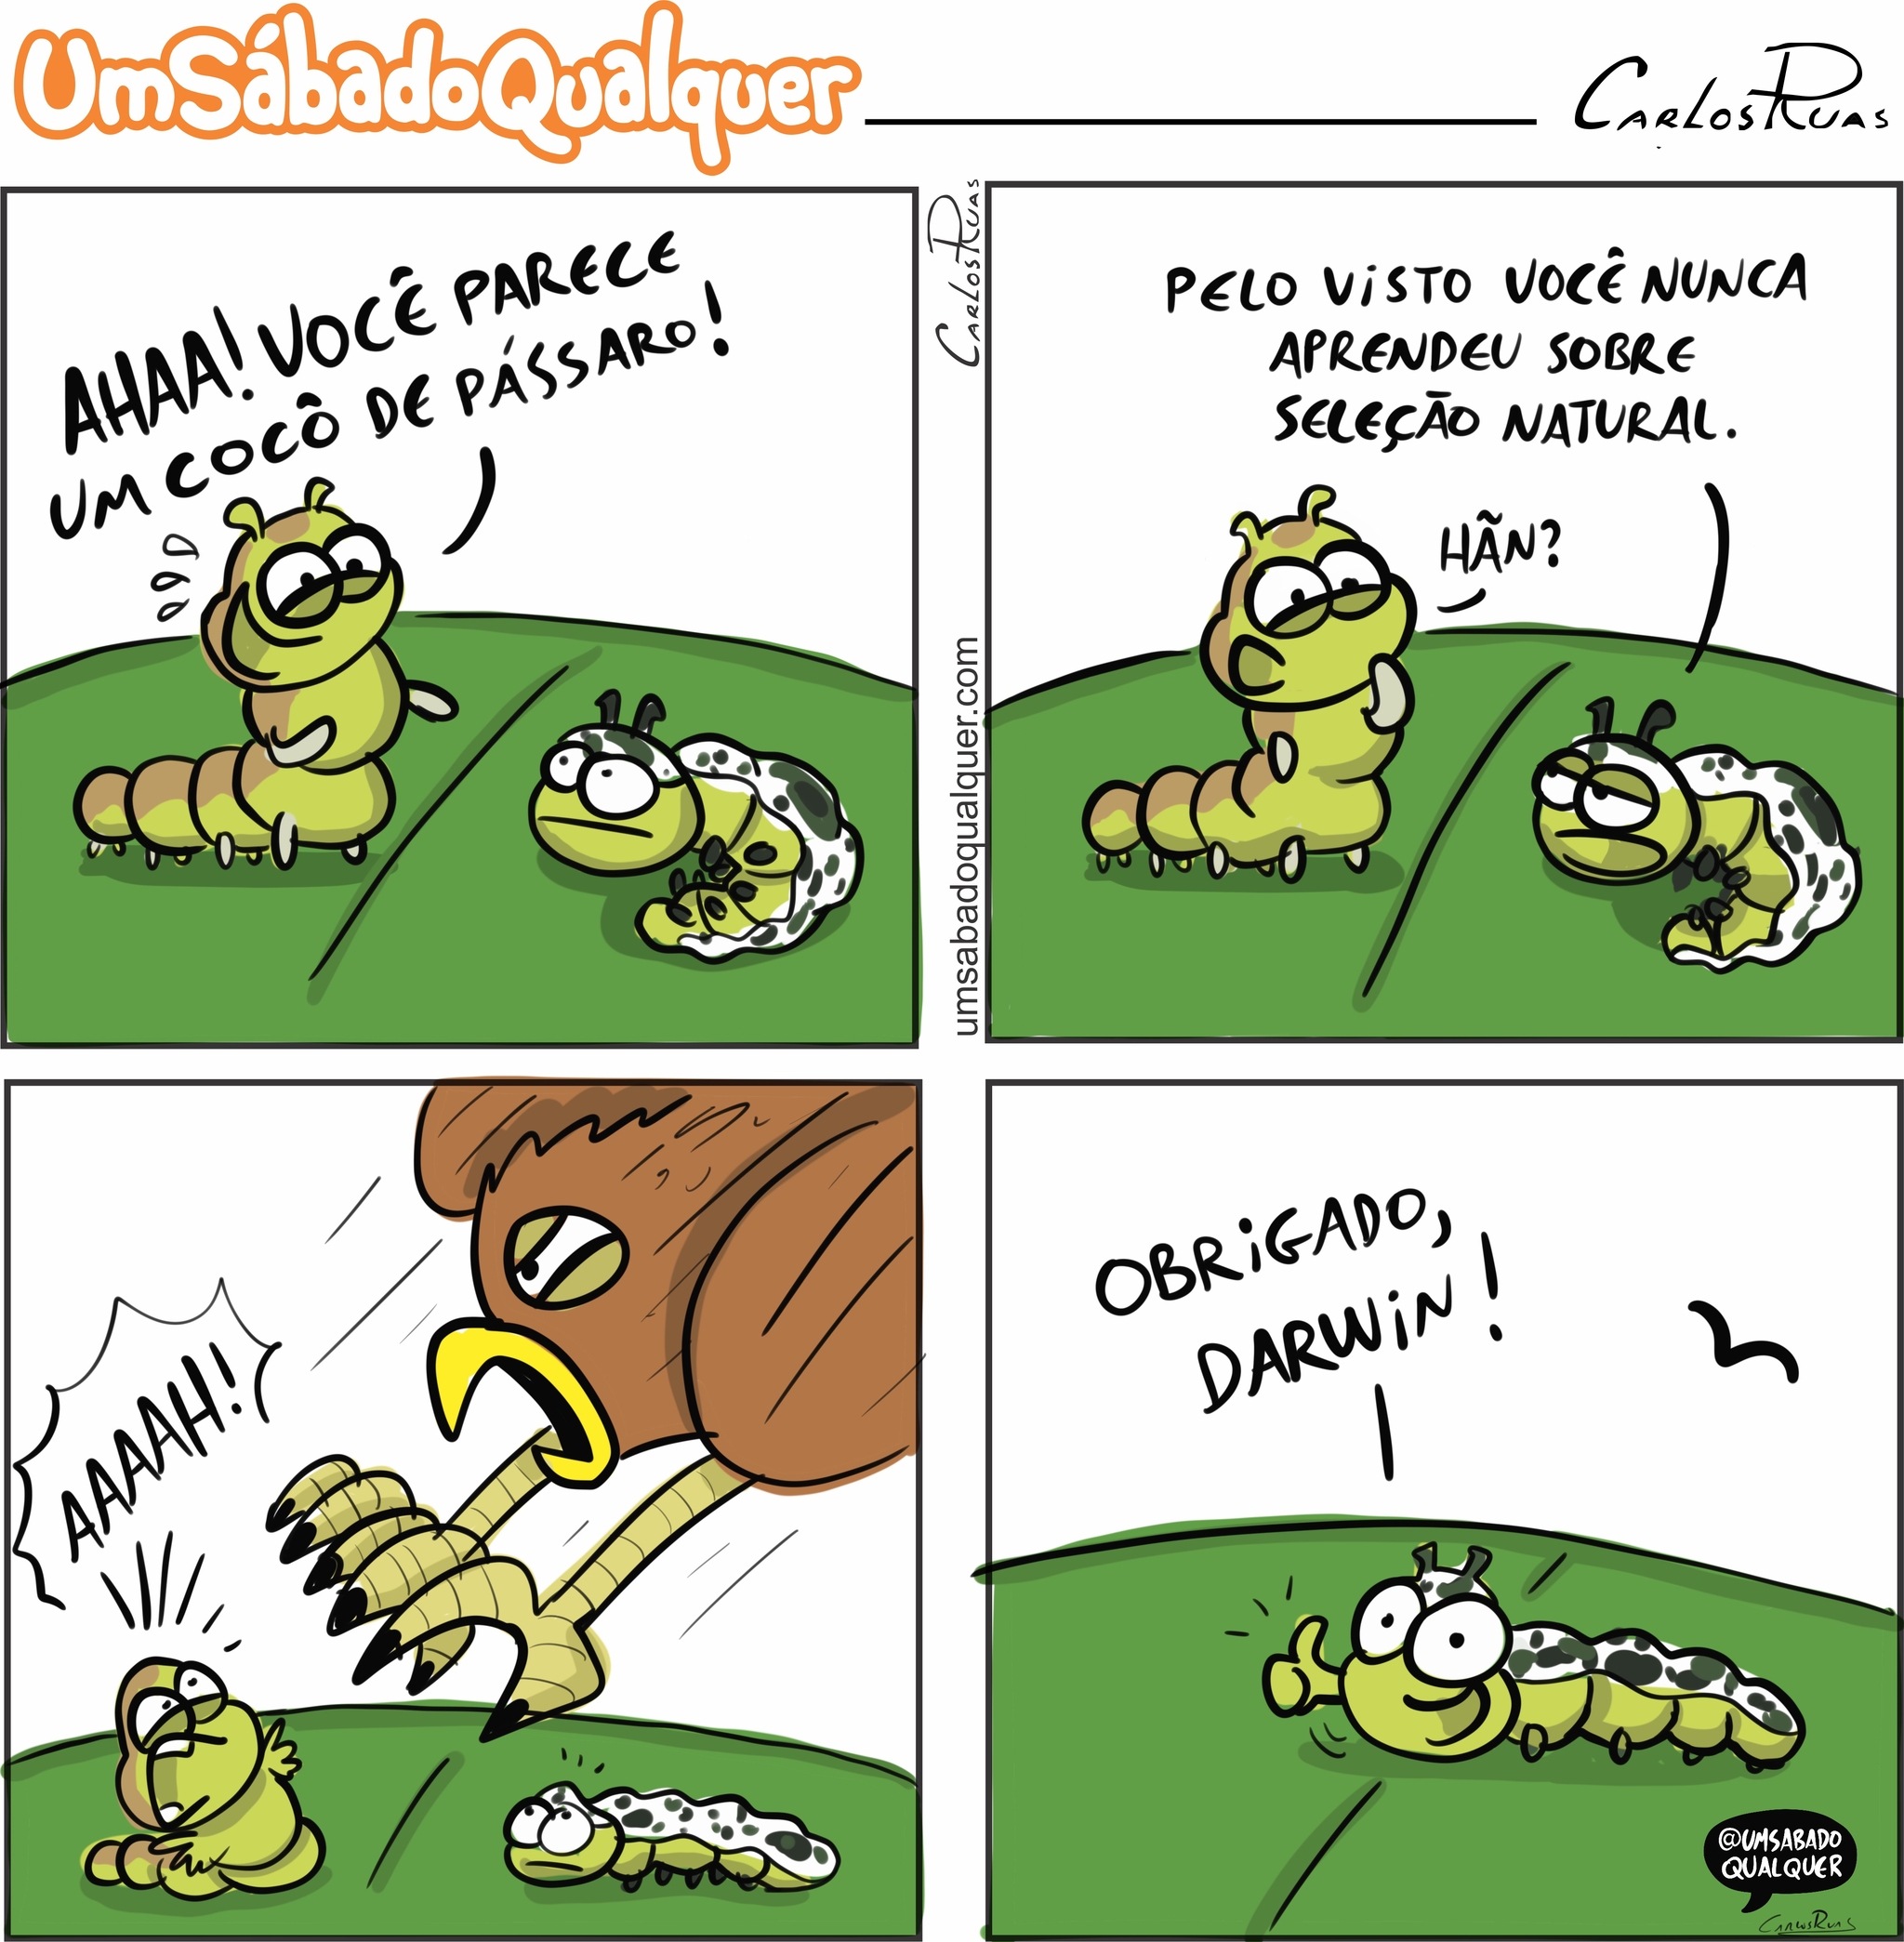
\includegraphics[width=.8\textwidth]{./images/PNLD0060-11}
\captionof{figure}{Tirinha cômica sobre a teoria darwiniana da seleção natural. Disponível em umsabadoqualquer.com}

	\item
	É interessante que a produção da árvore do tempo, que poderá ser tanto física
	quando digital, contenha elementos do universo dos e das estudantes, como 
	a o exemplo da tirinha a seguir compartilhada nas redes sociais. Desta forma,
	com a aproximação da linguagem, o conteúdo chegará com maior facilidade. 


\end{enumerate}




\section{Aprofundamento}

Nesta seção, desenvolvemos um trabalho de aprofundamento que, em diálogo com
a formação continuada de professores, oferece subsídios para a abordagem do
texto literário. A leitura em sala de aula de \emph{A origem das espécies} pode
ser enriquecida pelo aprofundamento no universo literário em que a obra está
inserida.

\subsection{A obra}

\emph{A origem das espécies} se fez uma obra revolucionária desde sua primeira edição.
Publicada em 1859, a obra detém os louros de, apesar de ser um
trabalho de literatura científica, ter sido produzido direcionado ao público
leigo, ofertando à população a teoria da seleção natural proposta por Charles
Darwin, oriunda de suas observações, e também de discussões e pensamentos que
há algum tempo já apresentavam certa efervescência na comunidade científica.

Rapidamente, o livro se tornou um sucesso e motivo de controvérsia. Isso se
deve ao fato de que a proposta de modificação das espécies contrariava
conhecimentos clássicos e interpretações de textos religiosos. O debate gerado
ocasionou uma maior independência das ciências e um amadurecimento da
metodologia científica, entretanto, o próprio trabalho de Darwin foi deixado de
lado em função de outras obras que foram, em um primeiro momento, melhor
aceitas.

Tais teorias, no entanto, foram rapidamente falseadas, recebendo a teoria de
Darwin seu lugar de direito anos mais tarde.

A obra é grandiosa por propor o princípio da seleção natural, esclarecendo como
pressões no ambiente ocasionam mudanças nos indivíduos e, por sua vez, alteram
toda uma população. Ela também merece destaque por ter fomentado um sistema que
se mostrou aplicável e consoante a descobertas futuras, de modo que, quanto
mais se pesquisa acerca do desenvolvimento da vida no planeta terra, mais se
confirmam os mecanismos propostos por Charles Darwin.


\subsection{Viagem pelo mundo}

O próprio Darwin inaugura sua obra indicando o impacto que a viagem a bordo do
HMS Beagle causou em si e como a mesma foi basilar para a produção de sua
teoria.


\Image{Ilustração da viagem marítima. (Alex Cerveny; Direitos cedidos à Ubu)}{PNLD0060-05.png}


A viagem ocorre em razão do contexto de sua época, em que o Império Espanhol
havia ruído, acabando com o monopólio de Madri no Hemisfério Ocidental. Somado
a isso, fazia-se necessária a atualização das cartas de navegação, muitas vezes
equivocadas ou incompletas.

Assim, o HMS Beagle partiu de Plymouth, Reino Unido, com objetivo de determinar
rotas seguras para o comércio, singrando, inicialmente, pelas águas do
Atlântico, visando atingir a América do Sul, para depois iniciar a navegação ao
redor do Globo, retornando, por fim, ao porto de onde partira.


\Image{Estrutura do navio Beagle (Alex Cerveny; Direitos cedidos à Ubu)}{PNLD0060-04.png}


No decorrer da viagem, em todas as paradas que faziam em terra firme, Charles
Darwin percorria longos trajetos a pé realizando anotações e desenhos em seus
caderninhos. Em uma dessas rondas, nas ilhas Galápagos - Equador, Darwin
observa que os Tentilhões da Ilha Floreana eram distintos dos vistos em outros
locais do arquipélago. Muitos predicam essa observação como momento de
epifania, onde Darwin começara a construir sua Teoria da Evolução.

\subsection{Descoberta compartilhada}

No início de 1858, Darwin recebeu a correspondência de um colega naturalista de
nome Alfred Russel Wallace, em que este relatava estudos que havia realizado em
uma viagem pelos arquipélagos do Sudeste Asiático. Neles, Wallace indicava
o princípio da seleção natural com modificação, ocasionada pela batalha dos
seres vivos pela sobrevivência.

Ou seja, conclusões muito próximas àquelas que Darwin vinha estudando nas
últimas duas décadas. A correspondência, juntamente com outros dois escritos de
Darwin, que mais tarde culminariam em \emph{A Origem das Espécies}, foram lidas
diante dos pares dos naturalistas na Linnean Society de Londres. Da leitura
e de posterior deliberação, a sociedade optou por dar prioridade à teoria de
Darwin, considerando-a mais bem fundamentada. Fato que fora reconhecido pelo
próprio Wallace.


\Image{Diagrama de ramificação dos roedores e marsupiais a partir de uma mesma
matriz. Década de 1850. (Charles Darwin; Domínio Público)}{PNLD0060-07.png}


A descoberta compartilhada dos mecanismos da seleção natural com modificação
é um ponto de inflexão na história da humanidade. E só foi possível por ser
produto de uma elaboração científica perene e eficiente, somada às
possibilidades que a tecnologia havia conferido ao homem da época, no sentido
de tornar possível as viagens de grandes distâncias.


\Image{Esquema geral de ramificação das espécies por seleção natural. Década
de 1840. (Charles Darwin; Domínio Público)}{PNLD0060-06.png}


\subsection{Ombros de gigantes}

Conta a história que Isaac Newton, comentando acerca de seu prolífico trabalho,
afirmou que só conseguira enxergar mais longe que a média por ter se apoiado
nos ombros de gigante. Com essa metáfora, o grande cientista inglês pretendia
dizer que suas descobertas só foram possíveis graças ao trabalho de outros
cientistas importantes anteriores a Newton, cujas produções serviram de base
para as teorias newtonianas.

Essa reflexão de Newton também pode ser aplicada a seu conterrâneo naturalista.
Na terceira edição de \emph{A origem das espécies}, o próprio Darwin traça um
caminho histórico de sua evolução, prestando a devida homenagem a outros
cientistas que vieram antes dele, como Jean-Baptiste Lamarck e Étienne Geoffroy
Saint-Hilaire.

O conceito de classificação em espécies, a ideia de modificação de acordo com
o meio, a ideia de um germe primordial único, são todos pensamentos anteriores
nos quais Darwin bebeu e, seguramente, conferiram-lhe um caminho e certa
clareza na análise de suas observações.

E se Darwin subiu no ombro de gigantes, certamente serviu de apoio a outros que
viriam depois de si. Sem os trabalhos de Charles Darwin (conjuntamente aos de
Gregor Mendel), seriam impossíveis as descobertas de Watson e Crick e de
Dobzhansky, fundamentais aos conhecimentos teóricos de genética, bem como suas
aplicações práticas.

\subsection{Base para a ecologia}

Um dos pontos principais da Teoria da Evolução é aquele que indica que os seres
respondem ao meio-ambiente. Melhor dizendo, o meio-ambiente gera nos indivíduos
uma pressão seletiva, a partir da qual, apenas os melhores adaptados a essas
condições sobrevivem. E os sobreviventes tem maior chance de passar seus genes
adiante, de modo que sua descendência herda suas características. O que, no
longo prazo, gera modificações nas populações, ocasionando em espécies
distintas.

Pois bem, em muitos casos, há uma especialização tão aguda das espécies que,
pequenas alterações no meio-ambiente, são capazes de causar grande impacto na
sobrevivência desses seres, podendo gerar, inclusive, extinção de populações
inteiras.

Nos últimos séculos registramos que a poluição do ar, das águas, a introdução
de espécies exóticas, vegetais e animais, em ecossistemas há muito
estabelecidos causaram grande desequilíbrio ecológico, gerando por vezes
o desaparecimento completo de espécies e o fim desses ambientes de vida.

Graças a Darwin, sabemos que isso não ocorre por mero acaso. Darwin legou
a humanidade a base para conhecermos a delicadeza de um dos princípios da vida
em nosso planeta -- até então, único lugar que conhecemos a abrigá-la --,
fazendo, indiretamente, com que também compreendêssemos que nós também somos
tão frágeis quanto outras espécies, e que ataques constantes ao ecossistema
podem levar à nossa própria desagregação.

\subsection{Por que ler \emph{A origem das espécies}?}

\emph{A origem das espécies} é uma obra que se tornou fundamental em toda
a ciência. A partir dos mecanismos nela descritos, abre-se um universo diante
do leitor, por meio do qual é possível compreender os caminhos que a vida tomou
desde seu surgimento no planeta Terra.

Assim, a obra é base para o entendimento da vida, do conceito de evolução e suas
aplicações, sendo até hoje referência no assunto.

O brilhantismo da obra reside não apenas na riqueza de suas proposições, mas
também, em sua simplicidade. Tendo sido escrita pensando no público em geral,
a obra foge aos termos por demais complexos ou conceitos por demais abstratos,
tornando o grande conhecimento que oferta palatável à todas as pessoas.


\subsection{Atividades para o aprofundamento da pesquisa}

No Ensino Médio, da mesma forma que no Ensino Fundamental, a BNCC organiza
o trabalho com as práticas de linguagem em cinco campos de atuação
social. São eles: campo da vida pessoal, campo da vida pública, campo
jornalístico-midiático, campo artístico-literário e campo das práticas de
estudo e pesquisa.

De acordo com essa divisão, propomos na sequência um trabalho interdiscursivo
e intertextual com a obra \emph{A origem das espécies}.
	
%\subsection{Campo da vida pessoal}
\subsubsection{Minidocumentário de
      divulgação científica}

Darwin chegou a ser muito contestado em sua época, porque
      havia um ponto muito problemático em sua teoria: a ideia de que o homem
      não figurava em um lugar distinto da escala evolutiva, sendo apenas mais
      um produto de milhões de anos de evolução. Apesar de todas as
      comprovações científicas à sua proposição, muitas pessoas ainda contestam
      a obra de Darwin. Contestar faz bem, é o caminho para o crescimento
      científico. Entretanto, isso deve ser pautado em dados, em pesquisa
      séria, e não em simples opiniões. Contudo, com as redes sociais,
      permitiu-se que quem detivesse maior exposição midiática fosse capaz de
      atingir mais pessoas com suas crenças, não sendo elas necessariamente
      científicas. Na contemporaneidade vive-se o problema das \emph{fake
      news}, comumente transmitidas por aplicativos, que acabam por gerar
      pânico e desinformação. Para abordar essa questão, divida a turma em
      pequenos grupos e proponha a produção de um minidocumentário de
      divulgação científica sobre o perigo das notícias falsas, abordando os
      riscos que as mesmas geram à sociedade. 
      \BNCC{EM13LP17}

Os alunos podem utilizar aplicativos gratuitos de gravação
  e edição de vídeos, disponíveis em dispositivos digitais, para montar um
  vídeo de até 4 minutos sobre o tema. É possível utilizar desenhos
  e animações, formato de telejornal ou de \emph{vlog}, com cuidados para
  garantir qualidade de áudio e imagem. Reforce a importância de haver um
recorte histórico-cultural do tema.

%\subsection{Campo de atuação na vida pública}
\subsubsection{Políticas de direito e respeito aos animais}

O entendimento jurídico sobre os animais vem paulatinamente sendo
mudado. De seres semoventes, os animais passaram a ser seres sencientes.
Ora, isso reflete um anseio da sociedade que passou a ver os bichos como
amigos, e não mais como instrumento de trabalho, ou de alimentação.
Recomenda-se, nessa atividade, que os alunos reflitam sobre a questão
e avaliem se há políticas de direito e respeito aos animais em suas
comunidades. Observando isso, os alunos devem redigir um manifesto ou carta
simbólica a autoridades locais, solicitando maior atenção à questão.
\BNCC{EM13LP27}

%\subsection{Campo jornalístico-midiático }
\subsubsection{Um texto investigativo-jornalístico}

A leitura de \emph{A origem das espécies} permitiu aos
      alunos entrarem em contato com conceitos como pressão seletiva. Assim
      sendo, eles hoje já têm consciência de que alterações no meio-ambiente
      provocam mudanças no bioma. Como algumas espécies são mais sensíveis
      a essa mudança, qualquer pequena modificação pode gerar sua
      extinção. Na mídia, muito se debate acerca das questões ambientais.
      Entretanto, os alertas nem sempre são observados. Esta atividade propõe
      que os alunos façam um texto investigativo-jornalístico sobre os impactos
      ambientais. Pegando, para isso, notícias de jornais, vídeos, dados de
      pesquisa, gráficos, que corroborem o texto escrito. O resultado final
      poderá ser publicado no jornal da escola ou no site do colégio.
      \BNCC{EM13CNT203}

%\subsection{Campo artístico-literário }
\subsubsection{Um registro fotográfico}

Retome com os estudantes a importância do desenho dentro
      das obras de Darwin e de outros naturalistas. Posteriormente, aconselhe
      os alunos a buscarem outros desenhos de viajantes, fotografias e mesmo
      pinturas de outros tempos. Um exemplo do último item sugerido é o artista \href{https://www.artyfactory.com/art_appreciation/animals_in_art/albrecht_durer.htm}{Albrecht Dürer} (1471--1528). 

      É interessante realizar um antes e um depois
      entre os locais que essas imagens retratam e a atualidade. Com isso será
      possível apresentar para os alunos os efeitos da passagem do tempo,
      que tenhamos conhecimento de como era o mundo no passado
      e até mesmo tenhamos a visualização de espécies que já foram
      extintas. 

      Feito isso, convide os alunos a fazerem um registro fotográfico
      de elementos de seus cotidianos. A rua da escola, o caminho que fazem
      para chegar ao colégio, as plantas e aves de um jardim próximo. Se
  possível, aconselha-se também a pesquisa de outras imagens de como foram
  esses locais no passado.
\BNCC{EM13LP18}

%\subsection{Campo das práticas de estudo e pesquisa}
\subsubsection{Evolução, microbiologia e genética}

Proponha uma pesquisa para ampliação do repertório acerca
      da evolução, microbiologia e genética. Para isso, recomenda-se a divisão
      da sala em grupos, para promover um congresso científico, onde os alunos
      irão expor as mais recentes descobertas desses campos. Como por exemplo,
      podemos citar o \textsc{crispr}, os chamados \textsc{dna} vestigiais, a influência de
      vírus na composição de nosso \textsc{dna}, etc. Cada exposição deve contar com uma
      apresentação com dados e imagens e incentiva-se os alunos para que
  fomentem o debate após as apresentações.  
\BNCC{EM13LP16}


\section{Sugestões de referências complementares}

\subsection{Filmes}

\begin{itemize}

\item \emph{Criação}. Direção: John Amiel, 2009.

O filme foi baseado no livro \emph{Annies’s Box}, escrito pelo tataraneto de Darwin e acompanha os momentos que antecederam a publicação de \emph{A origem das espécies} e os conflitos existenciais que afligiram seu autor em vias de divulgá-lo. 

\item \emph{Mestre dos mares --- o lado mais distante do mundo.} Direção: Peter Weil, 2003.

O filme se passa durante as Guerras Napoleônicas e conta a história de um capitão de um navio de guerra britânico. 
Há uma analogia aos estudos de Darwin em um trecho do filme, em que a personagem Doutor Stephen Maturin relata as adaptações ocorridas em algumas espécies para sobreviverem nas Ilhas Galápagos.

\item \emph{O desafio de Darwin}. Direção: John Bradshaw, 2009.

O filme conta a história dos conflitos que Darwin viveu em 1858,
logo antes de publicar \emph{A origem das espécies}. 

\item \emph{Wall-E}. Direção: Andrew Stanton, 2008.

A animação da Pixar confabula sobre o mundo após a destruição da Terra, que em que a humanidade deixou o planeta e foi viver em uma nave.

\end{itemize}

\subsection{Séries}

\begin{itemize}
\item \emph{Evolução para todes.} Direção: Ivanildo Soares, 2021

Série animada do \href{https://www.youtube.com/watch?v=d_4hLpzRh1A}{Canal USP}, parte da pergunta "de onde viemos?" para estimular crianças e jovens a se interessarem por ciência, arqueologia, antropologia e evolução humana.

\item \emph{Mundo mistério.} Direção: Felipe Castanhari, 2020.

Série da Netflix acompanha o apresentador Felipe Castanhari, que explora os mistérios da ciência e da história,
com temas como superinteligência artificial, viagem no tempo, aquecimento global, entre outros.

\item \emph{Seleção artificial.} Direção: Joe Egender e Leeor Kaufman, 2019.

A série da Netflix acompanha cientistas na descoberta das modificações de \textsc{dna},
seja para erradicar doenças ou escolher características de bebês.

\end{itemize}

\subsection{\emph{Sites}}

\begin{itemize}

\item Biblioteca do Instituto de Biociências da USP

A \href{https://biblioteca.ib.usp.br/}{biblioteca} possui um extenso arquivo de artigos científicos, livros, teses acadêmicas, entre outros.

\item Manual do Mundo

Canal do \href{https://www.youtube.com/user/iberethenorio}{Youtube} com vídeos diversos sobre experimentos científicos e criativos.
\end{itemize}


\subsection{Museus}

\begin{itemize}

\item Museu Biológico do Instituto Butantan

O museu conta com uma exposição zoológica viva e permanente. Lá podem ser vistos serpentes, aranhas, escorpiões, lagartos, peixes e insetos, em recintos que recriam seu habitat natural.

\item Museu Catavento

Espaço interativo que apresenta a ciência de forma dinâmica e interativa para crianças, jovens e adultos. Foi o Museu mais visitado do Estado de São Paulo por três anos consecutivos.

\item Museu do Amanhã

Localizado na Praça Mauá, no centro do Rio de Janeiro, o Museu do Amanhã busca ser um museu de ciências diferente e oferece, com projeções de vídeos e mesas interativas, uma narrativa sobre como poderemos viver e moldar os próximos 50 anos. 

\end{itemize}

\section{Bibliografia comentada}

\begin{itemize}
\item \textsc{browne}, Janet. \emph{A origem das espécies de Darwin: uma biografia.}  Rio de
Janeiro: Zahar, 2007.

A autora apresenta a história da composição e os principais conceitos
presentes em \emph{A origem das espécies}, com contextualização
histórico-cultural do universo de Charles Darwin.

\item \textsc{darwin}, Charles. \emph{A expressão das emoções no homem e nos animais.} São
Paulo: Companhia de Bolso, 2009.

Em uma de suas obras mais acessíveis, Darwin demonstra que os animais também
sentem raiva, medo, ciúmes, manifestados por meio das expressões, que ele
analisa do ponto de vista de sua funcionalidade na adaptação do indivíduo ao
meio.

\item \textsc{darwin}, Charles. \emph{Viagem de um naturalista ao redor do mundo, volumes
1 e 2}. São Paulo: L\&PM, 2008.

Estes dois volumes compilam os diários escritos pelo naturalista britânico
durante a icônica expedição de cinco anos a bordo do navio Beagle, iniciada
quando ele tinha apenas 22 anos.


\item \textsc{dawkins}, Richard. \emph{O gene egoísta}. São Paulo: Companhia das Letras,
2007.

Este clássico da divulgação científica apresenta a biologia evolutiva de forma
acessível e lança a interpretação de que somos máquinas de sobrevivência
a serviço dos genes.

\item \textsc{hippel}, William von. \emph{A evolução improvável}. Rio de Janeiro: Harper
Collins, 2019.

O psicólogo cruza a ciência evolutiva com diversas áreas do conhecimento para
mostrar como eventos do passado distante influenciam nossas vidas.  Com essas
ferramentas, procura explicar questões como por que exageramos e por que
acreditamos em nossas mentiras.

\item \textsc{lopes}, Reinaldo José. \emph{Darwin sem frescura}. Rio de Janeiro: Harper
Collins, 2019.

O livro é um mergulho descontraído na teoria da Evolução, buscando responder
questões em torno dela: De onde veio nossa espécie? A humanidade está em
processo de extinção? Por que irlandeses têm mais tolerância à lactose do que
chineses?

\item \textsc{sagan}, Carl. \emph{Cosmos}. São paulo: Companhia das Letras, 2017.

Este \textit{best"-seller} retraça 14 bilhões de anos de evolução cósmica, discutindo
temas como a origem da vida, hieróglifos egípcios, missões espaciais, a morte
do sol e a evolução das galáxias.
\end{itemize}

\end{document}


